\documentclass{homework}
\usepackage{xcolor}
\usepackage{nicematrix}
\usepackage{booktabs}
\usepackage{enumitem}
\usepackage{caption}
\usepackage{subcaption}
\usepackage{leftidx}
\usepackage{mathrsfs}
\usepackage{pgfplots, pgfplotstable}

\NiceMatrixOptions{cell-space-limits = 1pt}

\title{Simulation and Modeling I, Assignment 1}
\author{
  Dmitrii, Maksimov\\
  \texttt{dmitrii.maksimov@fau.de}
  \and
  Priyanka, Muddarla\\
  \texttt{priyanka.muddarla@fau.de}
  \and
  Susmitha, Palla\\
  \texttt{susmitha.palla@fau.de}
  \and
  Bhaskar Jyoti, Gogoi\\
  \texttt{bhaskar.j.gogoi@fau.de}
}

\makeatletter
\long\def\ifnodedefined#1#2#3{%
    \@ifundefined{pgf@sh@ns@#1}{#3}{#2}%
}

\pgfplotsset{
    discontinuous/.style={
    scatter,
    scatter/@pre marker code/.code={
        \ifnodedefined{marker}{
            \pgfpointdiff{\pgfpointanchor{marker}{center}}%
             {\pgfpoint{0}{0}}%
             \ifdim\pgf@y>0pt
                \tikzset{options/.style={mark=*}}
                \draw [densely dashed] (marker-|0,0) -- (0,0);
                \draw plot [mark=*, mark options={fill=white}] coordinates {(marker-|0,0)};
             \else
                \tikzset{options/.style={mark=none}}
             \fi
        }{
            \tikzset{options/.style={mark=none}}        
        }
        \coordinate (marker) at (0,0);
        \begin{scope}[options]
    },
    scatter/@post marker code/.code={\end{scope}}
    }
}

\makeatother


\begin{document}

\maketitle

\exercise
\begin{enumerate}[label=(\alph*)]
	\item At a multi-port switch S, packets may arrive via four different input ports P1, \dots, P4 and are switched to different output ports. The table below shows which percentage/share of the arriving packets each input port carries and the switching error probability for each input port.
		\begin{center}
		    	\begin{tabular}{| l | l | l |}
		    	\hline
			    input port & share of arriving packets & switching error probability \\ \hline
			    P1 & 55\% & 0.077 \\ \hline
			    P2 & 5\% & 0.0001 \\ \hline
			    P3 & 17\% & 0.15 \\ \hline
			    P4 & 23\% & 0.002 \\
			\hline
			\end{tabular}
		\end{center}
	\textbf{What is the probability that an arbitarary arriving package is switched correctly?}
	
	Let \emph{A} be the event that an arbitrary arriving packet is switched correctly and \emph{B} be the input port, then using the law of total probability: \[P(A)=\sum_{i=1}^4 P(A|B=P_i)P(B=P_i).\] Taking into account that $P(A|B=P_i) = P(C'|B=P_i)$, where C is an event that packet switched incorrectly:
\[P(A) = (1-0.077)\cdot 0.55 + (1-0.0001)\cdot 0.05 + (1-0.15)\cdot 0.17 + (1-0.002)\cdot 0.23 = 0.931685.\]
	\item Now consider two such multi-port switches S1 and S2 connected in such a way that all packets of input port P1 on the first switch S1 are switched so that they enter switch S2 on its input port P1 (we don’t care about other traffic!). We are interested in the probability that packets along this single path are received correctly after switch S2. (We assume perfect links, i.e., packets are not lost between switches.)

\textbf{What is this probability}
\begin{itemize}[label={--}]
	\item \textbf{if both switches are independent?}

	Let \emph{D} - be the event that packets are received correctly after switch S2, then the only possible way is when both are swithed successfully:
	\[P(D) = P(A|B=P_1)(P(A|B=P_1) = (1-0.077)\cdot (1-0.077) = 0.851929.\]
	\item \textbf{if a transmission on S2 is always successful on the condition that the transmission on S1 was successful?}

	In this case if the transmission only on S1 is successful then packets are received correctly. Hence, \[P(D) = P(A|B=P_1) = (1-0.077) = 0.923.\]
\end{itemize}
\end{enumerate}
\exercise*
Are two disjoint events \emph{A} and \emph{B} with $P(A) > 0$ and $P(B) > 0$ stochastically independent of one another? Give both a formal and an informal answer! („Informal“ means to give the answer in your own words as opposed to formulas.)
\begin{itemize}
\item formal answer

Let \emph{A} and \emph{B} be the disjoints events then $P(A\cap B) = 0$. If \emph{A} and \emph{B} are also independent then $P(A\cap B) = P(A)\cdot P(B) = 0$. It is possible only if \emph{P(A) = 0} or \emph{P(B) = 0} which contradicts the condition. Hence, \emph{A} and \emph{B} aren't independent.

\item informal answer

Suppose you flip a coin. The coin lands on head(event A) or on tail(event B). Event A and event B would be disjoint because they both cannot occur at the same time. The coin cannot land on head and tail. So, if a A and B would be independent events it would be possible to observe both head and tail in one flip, but if event A has happend then there is no possibility to observe event B. Hence, these are dependent events.
\end{itemize}

\exercise*
Given the following experiment:

You have a box with 2 blue and 2 red balls inside. You blindly pick a ball, note its color and put it aside (not back into the box!). After that, you pick another ball from the box. Each pick gives you either a “Red” (R) or “Blue” (B) ball.
\begin{enumerate}[label=(\alph*)]
	\item \textbf{Set up the probability space ($\Omega$, $\mathcal{F}$, $P$)}

	$\Omega = \{RR, RB, BR, BB\}$

	$\mathcal{F} = \{\emptyset, \Omega\, \{RR\}, \{RB\}, \{BR\}, \{BB\}, \{RB, BR, BB\}, \{RR, BR, BB\}, \{RR, RB, BB\}, \{RR, RB, BR\},\newline \{RR, RB\}, \{RR, BR\}, \{RR, BB\}, \{RB, BR\}, \{RB, BB\}, \{BR, BB\}\}$
	
	Probability function \emph{P} for each each event in $\mathcal{F}$:
	\begin{itemize}
		\item $P(\emptyset) = 0$
		\item $P(\Omega) = 1$
		\item $P(\{RR\}) = P(R_1)\cdot P(R_2|R_1) = \frac{2}{4}\cdot \frac{1}{3} = \frac{1}{6}$
		\item etc.
	\end{itemize}
	\item \textbf{Define random variable X: S $\rightarrow$ R} such that \emph{X} denotes the number of occurences of the event „Red“ with respect to the experiment above!
	\begin{itemize}
		\item $X(RR) = 2$
		\item $X(RB) = 1$
		\item $X(BR) = 1$
		\item $X(BB) = 0$
	\end{itemize}
\item \textbf{Compute the full distribution function F(x)} for random variable X!
\begin{align*}
P(X\leq0) &= \dfrac{1}{4}\\
P(X\leq1) &= \dfrac{1}{4}+\dfrac{1}{2}=\dfrac{3}{4}\\
P(X\leq2) &= \dfrac{1}{4}+\dfrac{1}{2}+\dfrac{1}{2}=1
\end{align*}

{\centering
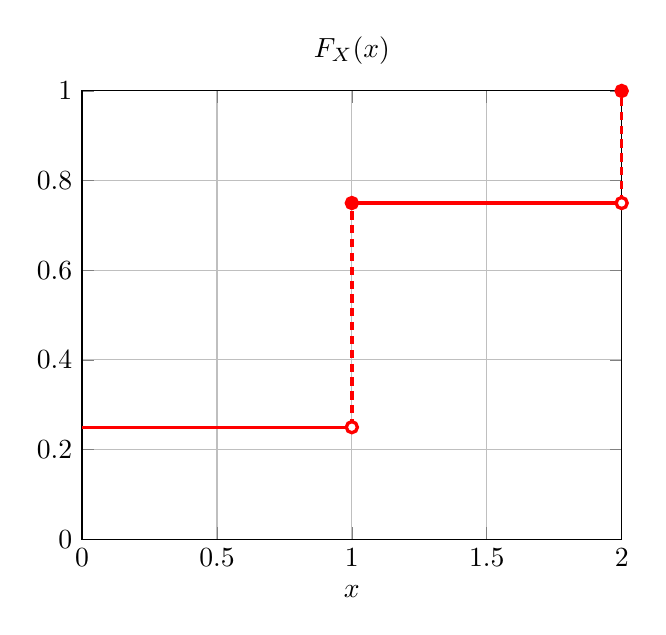
\begin{tikzpicture}
\begin{axis}[
    clip=false,
    jump mark left,
    ymin=0,ymax=1,
    xmajorgrids=true,ymajorgrids=true,
    xlabel={$x$},title={$F_X(x)$},
    xmin=0, xmax=2,
    every axis plot/.style={very thick},
    discontinuous,
    table/create on use/cumulative distribution/.style={
        create col/expr={\pgfmathaccuma + \thisrow{f(x)}}   
    }
]
\addplot [red] table [y=cumulative distribution]{
x f(x)
0 1/4
1 1/2
2 1/4
};
\end{axis}
\end{tikzpicture}
\par}
	
\end{enumerate}

\exercise*
A frequency-nonselective or flat fading radio channel may be accurately characterized by the Rayleigh model of fading. In this model, the received signal-to-noise ratio (SNR) per bit is described by an exponential distribution with density $f_{SNR}(x) = ce^{-cx}$, where parameter x is nonnegative $(x \geq 0)$ and c is some positive constant (c > 0). So, SNR is a random variable and $f_{SNR}(x)$ is indeed a density function for any value of c, since
\begin{itemize}
	\item $f_{SNR}(x) \geq 0, \forall x \geq 0 \text{ and } c > 0$
	\item $\int_{0}^{\infty} f_{SNR}(x) \,dx = 1, \forall c \in \R_{> 0}$ 
\end{itemize}
\begin{enumerate}[label=(\alph*)]
	\item \textbf{Determine the value of c} knowing that mean value of SNR is 35 dB!
	\begin{align*}
	E[SNR] &= \int_0^\infty x\cdot ce^{-cx}\,dx \\
	&= -(xe^{-cx}\big|_0^\infty - \int_0^\infty e^{-cx}\,dx) \\
	&= -xe^{-cx}\big|_0^\infty - \frac{1}{c} e^{-cx}\big|_0^\infty \\
	&=\frac{1}{c} = y,
	\end{align*}
where $35 = 10^{0.1y} \Rightarrow y \approx 15.4$. Hence, $c \approx \frac{1}{15.4}.$
	\item The probability of outage is an important performance criterion for digital communication over fading channels and is defined as the probability that the modem performs more poorly than a specified threshold. We require an SNR of at least 20 dB. Therefore, the probability of outage here is the probability that the SNR per bit is less than 20 dB. \textbf{What is the value of the probability of outage?}

	First, we find corresponding value for a threshold: $20 = 10^{0.1y} \Rightarrow y \approx 13.0$. Hence, the probability of outage is:
\begin{align*}
	P(X\leq13) &= \int_0^{13} ce^{-cx}\,dx \\
	&=-e^{-cx}\big|_0^{13} = -(e^{-\frac{13}{15.4}} - 1) \approx 0.57
\end{align*}
\end{enumerate}
\end{document}